%% modified for BE3M33UI at FEL CVUT
%% bare_jrnl.tex
%% V1.2
%% 2002/11/18
%% by Michael Shell
%% mshell@ece.gatech.edu
\documentclass[journal]{IEEEtran}
\usepackage{graphicx}


\begin{document}
%
% paper title
\title{B(E)3M33UI\\ Semestral project 1:\\Spam filter}
\author{Sinchiguano Cesar}


\markboth{SEMESTRAL WORK, COURSE BE3M33UI, CZECH TECHNICAL UNIVERSITY IN PRAGUE, 20018/19}{Shell \MakeLowercase{\textit{et al.}}: Bare Demo of IEEEtran.cls for Journals}
\maketitle

%done
\begin{abstract}
This paper explores and identifies the use of four different learning algorithms (Logistic Regression classifier, AdaBoost classifier, Random Forest classifier and Naive Bayesian Classifier) for classifying spam messages(spam filtering) from a data set. A comparative analysis of the algorithms has also been presented and it will showcase that simple AdaBoost classifier taking from the ensemble models, could
be efficient for the dataset which could be classified as binary tree.
\end{abstract}


%done
\section{Assignment}
The goal of this semestral task is to employ the knowledge of the ML lectures and previous exercises, and apply it to a text classification task, namely called spam filtering. A dataset with text
messages and their classification as spam or ham is provided, in addition to a skeleton code where it shows the use of a dummy classifier as the starting point. 

\section{Introduction}

The classification algorithms such as Logistic Regression classifier, AdaBoost classifier, Random Forest classifier and Naive Bayesian Classifier are currently used in various datasets and
showing a good classification result.

In this paper, the four algorithms already mentioned above are proposed as anti-spam filtering methods to compare their performances. For each algorithm, we develop it by adjusting some parameters better-called hyper-parameters to achieve its best possible predicted result with the use of Grid-search method.
Grid-search is a way to select the best of a family of models, parametrized by a grid of parameters. 

As to the data set. It was already divided into training and testing
sets. The way as it was dividing our data set is called cross-validation. And it is a good one approach in order to avoid the overfitting state. We then trained each one of the algorithms using the training set, and as for the last step, we proceeded to evaluate their performances on the testing set.
For the sake of the working algorithm, the training and testing sets had to be expressed as a vector. The dimensions in the vector are corresponding
to the word frequency existing in the document. To achieve that, we used the CountVectorizer method as the previous step to the training one. The CountVectorizer method converts from a text document to a matrix of token counts. The resulting matrix is composed of a number of each word appears in the text document. Therefore, we transformed our given inputs of a text domain into a numerical domain which can be treated as task classification using each on of the classification methods.

%%%%%%%%%%%%%%%%%%%%%%
%%%%%%%%%%%%%%%%%%%%%%
\begin{enumerate}
\item \textbf{Logistic Regression classifier}

Given a set of inputs X, we want to assign them to one of two possible categories (spam or ham). Logistic regression models the probability that each input belongs to a particular category. A function takes inputs and returns outputs. To generate probabilities, logistic regression uses a function that gives outputs between 0 and 1 for all values of X. There are many functions that meet this description, but the used in this case is the logistic function (sigmoid).

\begin{figure}[!h]
\begin{center}
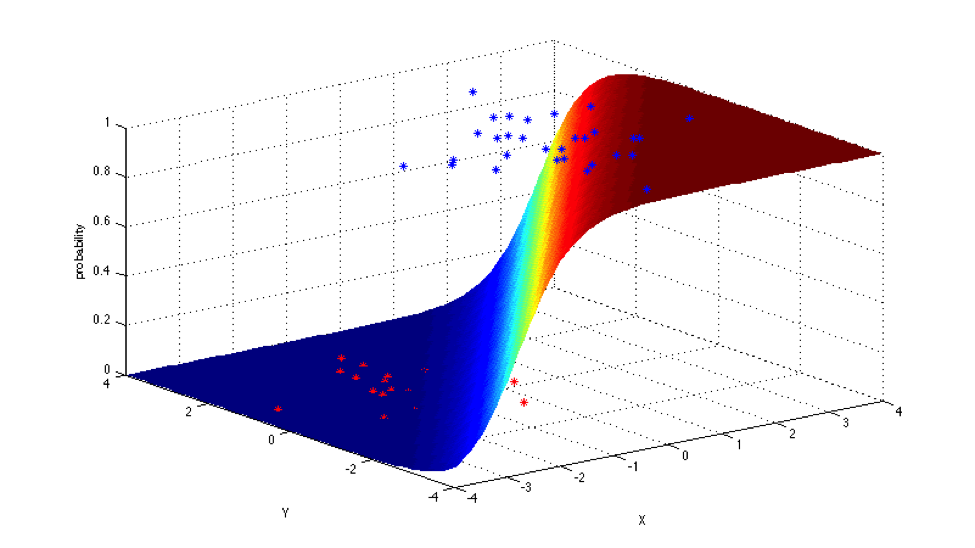
\includegraphics[width=2in]{fig2.png}
%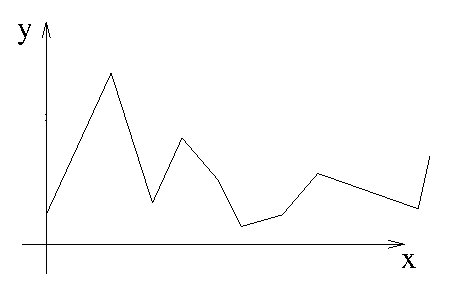
\includegraphics[width=2in]{figure.eps} %to texify use eps
\caption{An example of logistic regression. \cite{temp1}}
\end{center}\label{fig:mypicture}
\end{figure}


%%%%%%%%%%%%%%%%%%%%%%
%%%%%%%%%%%%%%%%%%%%%%
\item \textbf{AdaBoost classifier}

AdaBoost can be used to boost the performance of any machine learning algorithm. It is best used with weak learners. These are models that achieve accuracy just above random chance on a classification problem.

The most suited and therefore most common algorithm used with AdaBoost are decision trees with one level. Because these trees are so short and only contain one decision for classification, they are often called decision stumps.

Each instance in the training dataset is weighted. The initial weight is set to:

$$weight(x_i) = \frac{1}{n}$$

Where $x_{i}$ is the i’th training instance and n is the number of training instances.



%%%%%%%%%%%%%%%%%%%%%%
%%%%%%%%%%%%%%%%%%%%%%
\item \textbf{Random Forest classifier}

The random forest is another ensemble approach we used in this paper. The random-forest algorithm brings extra randomness into the model, when it is growing the trees. Instead of searching for the best feature while splitting a node, it searches for the best feature among a random subset of features. This process creates a wide diversity, which generally results in a better model.

\begin{figure}[!h]
\begin{center}
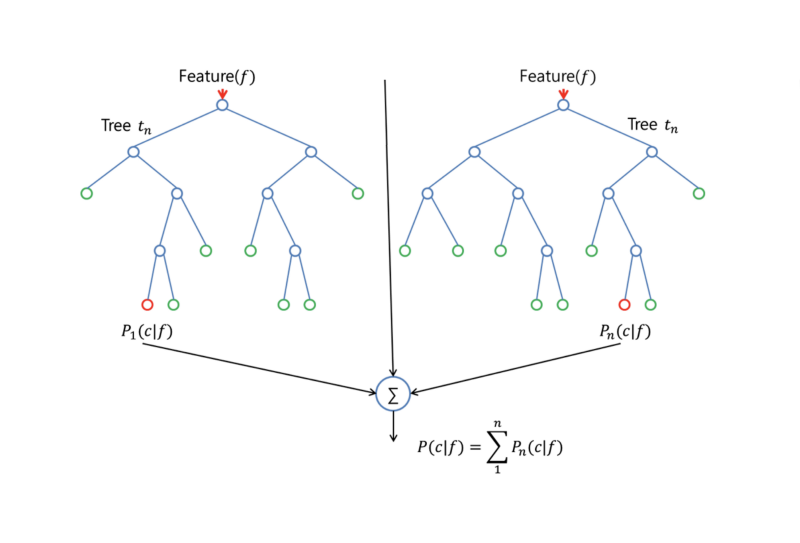
\includegraphics[width=2in]{fig3.png}
%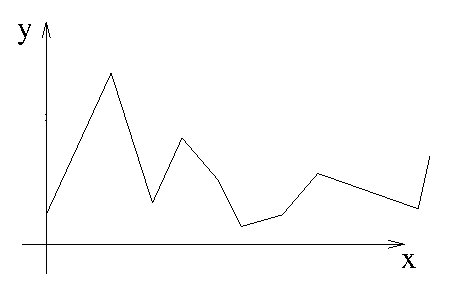
\includegraphics[width=2in]{figure.eps} %to texify use eps
\caption{An example of random forest with two trees. \cite{temp2}}
\end{center}\label{fig:mypicture}
\end{figure}

%%%%%%%%%%%%%%%%%%%%%%
%%%%%%%%%%%%%%%%%%%%%%
\item \textbf{Naive Bayesian (NB) Classifier}

Naive Bayesian algorithm is one of the frequently used
machine learning methods for text categorization. The original idea of identifying whether an email is spam or ham looking at which words are found in the message and
which words are absent from it. This approach begins by
studying the content of a large collection of emails which
have already been classified as spam or ham email.
Then when a new email comes into some user's mailbox,
the information obtained from the training set is used to
compute the probability that the email is spam or ham from
the words in the email.
Given a feature vector $ x =\{ x_{1},..., x_{n}\} $ where are the values of attributes $X_1 , . . ., X_n$ , and n is the number of attributes in the corpus. 
Let C denote the category to be predicted, i.e., $C \in \{spam,ham\}$. It uses a
discriminate function to compute the conditional probabilities of $P(C_i|X)$. Here, given the inputs, $P(C_i|X)$ denotes the probability that, example X belongs to class $C_i$ : 
$$P(C_i|X)=\frac{P(C_i)*P(X|C_i)}{P(X)}$$
$P(C_i )$ is the probability of observing class i. $P(X|C_i )$ denotes
the probability of observing the example, given class $C_{i}$.
$P(X)$ is the probability of the input, which is independent
of the classes.
\end{enumerate}

%%%%%%%%%%%%%%%%%%%%%%%%%%%%%
%%%%%%%%%%%%%%%%%%%%%%%%%%%%%%%


\section{Methodology}
%done
\begin{enumerate}
%\item Automatic tuning via grid search\\
\item \textbf{Automatic tuning via grid search}\\
All algorithms implemented have hyper-parameters. A hyperparameter is a parameter whose value is set before the learning process begins. By contrast, the values of other parameters are derived via training. When using any type of the classifier described above, default parameters are taking into account. However, these default parameters often times are not the right choice for optimal prediction of the algorithm. So that, we were obliged to change most of them, or at least the most important, those who can be suitable for the spam filtering task. 
There are two ways to do so, one of them can be done by hand, which can be a time-consuming task, the other alternative is to do it through an optimizer better known in Machine learning world as grid search where the algorithm is optimized by cross-validation based on a scoring function. The performance of the selected hyper-parameters and trained model is then measured on a dedicated evaluation set that was not used during the model selection step.
%not
%\item Model diagnostics
\item \textbf{Model diagnostics}

The modified accuracy macc is used to measure the quality of the several algorithms for the spam filtering task on a certain dataset. In addition to additional model evaluations such as Receiver operating characteristic (ROC) and AUC (which stands for Area under the curve) are discussed in order to better understand which spam filtering is performing well or not.

\end{enumerate}


%%%%%%%%%%%%%%%%%%%%%%%
%%%%%%%%%%%%%%%%%%%%%%%
%working on
\section{Experiments}

In this section, the four classification algorithms are evaluated the effects based on different hyper-parameters and also different feature sizes in order to find the optimal model for spam filtering. Afterward, the  performance of the spam filtering is measured in terms of accuracy. It means that each one of the filters is evaluated using a modified accuracy score which is already implemented in the supplied filter.py module as the function called $modified_{\_}accuracy$ which uses the confusion matrix feature to compute TP, FP, TN, FN.

$$macc=\frac{n_{TP}+n_{TN}}{n_{TP}+n_{TN}+10*n_{FP}+n_{FN}}$$

The algorithms described in the instroduction part, were carefully selected, not before a thorough research in many related jobs those who were done many years ago. Even so, in order to get a better and wide insight into the performance of each one of the models, we proceeded to run them with their default values, the results are shown in the Table \ref{modifiedaccuracy}. 

\begin{table}[ht]
\renewcommand{\arraystretch}{1.3}
\centering
\begin{tabular}{|c|c|}
\hline
Classifier & Accuracy score\\
\hline
Logistic regression & 70.75 \%\\
\hline
Adaboost & 70.75 \%\\
\hline
Random Forest & 64.39 \%\\
\hline
Naive Bayesian & 78.78 \% \\
\hline
\end{tabular}

\caption{Test accuracy of different classifiers with standard parameter-settings}
\label{modifiedaccuracy}
\end{table}

Table \ref{modifiedaccuracy} shows good performances for a Logistic regression, Adaboost and Naive Bayesian. On the contrary, Random forest performed badly as spam filtering, with that we confirmed the criterion of many researchers that Random Forest is not suitable for filtering spam messages and also that Naive Bayesian is more acute for the task. From now on, Random Forest classifier is irrelevant for a deeply study. Therefore, it is not dicussed anymore.

Considering as a first experiment the one we did above, running our model with default parameter, then we proceeded as a second experiment to run each model with the use an optimizer called grid search in order to find the best hyper-parameters for itself.

%in process
\begin{enumerate}

\item Logistic Regression classifier
\begin{enumerate}
\item Grid Search\\
We came out with four parameters: penalty, c, and class weight as parameters for the logistic regression classifier and $ngram_{\_}range$ as the only one parameter for the count vectorizer method. The reason to work with these exclusive parameters is that they are relevant in order to get a good result. We could use as many parameters as we wanted but the more we use them, the more time-consuming would be for the optimizer to find the best match. But it can be done if we could have worked with GPU which is suitable due to its high speed in processing data.  
 
\item Filter Evaluation\\
As we already mentioned in the methodology part, the filter is evaluated using the modified accuracy score. The results are shown in the Table \ref{temp0}

\begin{table}[ht]
\renewcommand{\arraystretch}{1.3}
\centering
\begin{tabular}{|c|c|c|}
\hline
$ Data$ & Default values & Tuned values\\
\hline
Training & 1.0 & 0.99167\\
\hline
Testing & 0.7076 & 0.8571\\
\hline
\end{tabular}
\caption{Accuracy score}
\label{temp0}
\end{table}
Table \ref{temp0} shows clearly that there is a significant improvement in the performance of the model. The table shows both scores, the one with default parameters and the other with the parameters found by the optimizer.

\item Best parameters

\begin{table}[ht]
\renewcommand{\arraystretch}{1.3}
\centering
\begin{tabular}{|c|c|}
\hline
$class_{\_}weight$ &  balanced\\
\hline
penalty & l2\\
\hline
$c$ & 0.1 \\
\hline
$ngram_{\_}range$ & (1, 3) \\
\hline
\end{tabular}
\caption{Hyper-parameters}
\label{temp2}
\end{table}
Table \ref{temp2} shows the final value of the hyper-parameters, those who were encounter by the grid search method.

\end{enumerate}

%%%%%%%%%%%%%%%%%%%%%%%%%%%%%
%%%%%%%%%%%%%%%%%%%%%%%%%%%%%

\item AdaBoost classifier


\begin{enumerate}
\item Grid Search\\
We came out with two parameters: $n_{\_}estimator$ for the AdaBoost classifier and $ngram_{\_}range$ as a parameter for the count vectorizer method.
 
\item Filter Evaluation\\
As we already mentioned in the methodology part, the filter is evaluated using the modified accuracy score. The results are shown in the Table \ref{temp0}

\begin{table}[ht]
\renewcommand{\arraystretch}{1.3}
\centering
\begin{tabular}{|c|c|c|}
\hline
$ Data$ & Default values & Tuned values\\
\hline
Training & 1.0 & 0.99167\\
\hline
Testing & 0.7075 & 0.83333\\
\hline
\end{tabular}
\caption{Accuracy score}
\label{temp0}
\end{table}
Table \ref{temp0} shows significant improvement in the perfomance of the model. The table also shows both scores, the one with default parameters and the other with the parameter found by the optimizer.

\item Best parameters

\begin{table}[ht]
\renewcommand{\arraystretch}{1.3}
\centering
\begin{tabular}{|c|c|}
\hline
$n_{\_}estimator$ & 30\\
\hline
$ngram_{\_}range$ & (1, 2) \\
\hline
\end{tabular}
\caption{Hyper-parameters}
\label{temp3}
\end{table}
Table \ref{temp3} shows the final value of the hyper-parameters, those who were encounter by the grid search method.
\end{enumerate}



%%%%%%%%%%%%%%%%%%
%%%%%%%%%%%%%%%%%%
\item Naive Bayesian Classifier\\
We select the MultinomialNB, which is one of the two classic naive Bayes variants used in text classification.

\begin{enumerate}
\item Grid Search\\
We came out with two parameters: alpha for Naive Bayesian classifier and $ngram_{\_}range$ as a parameter for the count vectorizer method.
The alpha determines how much the data should be smoothed and the $ngram_{\_}range$ decides between the following options: unigrams and $bi-grams$ in the model, in order to capture important information involving multiple tokens.
 
\item Filter Evaluation\\
As we already mentioned in the methodology part, the filter is evaluated using the modified accuracy score. The results are shown in the Table \ref{temp0}

\begin{table}[ht]
\renewcommand{\arraystretch}{1.3}
\centering
\begin{tabular}{|c|c|c|}
\hline
$ Data$ & Default values & Tuned values\\
\hline
Training & 1.0 & 0.99167\\
\hline
Testing & 0.7878 & 0.7988\\
\hline
\end{tabular}
\caption{Accuracy score}
\label{temp0}
\end{table}
Table \ref{temp0} shows slightly improvement. It was expected to work well enough for this kind of task due to its usage in many task related to spam filtering. 

\item Best parameters

\begin{table}[ht]
\renewcommand{\arraystretch}{1.3}
\centering
\begin{tabular}{|c|c|}
\hline
$n_{\_}estimator$ & 30\\
\hline
$ngram_{\_}range$ & (1, 2) \\
\hline
\end{tabular}
\caption{Hyper-parameters}
\label{temp5}
\end{table}
Table \ref{temp5} shows the final values of the hyper-parameters, those who were encounter by the grid search method.
\end{enumerate}
\end{enumerate}

%%%%%%%%%%%%%
%%%%%%%%%%%%%

\section{Discussion}

After the two experiments we did try on each one of the models. We are not able to tell which one should be selected, but it is clearly so far that logistic regression classifier performed well compare to the Adaboost classifier and the Naive Bayesian classifier. In order to take the final decision, we plot a Receiver operating characteristic curve better called ROC curve and we show the Area under the curve better known as AUC for each one of them.

\begin{enumerate}
\item Receiver Operating Characteristic curve\\
In order to choose the optimal model, we have to look carefully which curve is closer to the upper left corner of the fig. 3 and simultaneously we have to see which one is with the less false positive rate. And finally, we came out with the solution that the logistic regression is the one who meets the requirements. In Figure \ref{fig:mypicture}, we can also see the values of the area under the curve for each model in order to better confirm the selected model(logistic regression) as final spam filtering.

\begin{figure}[!h]
\begin{center}
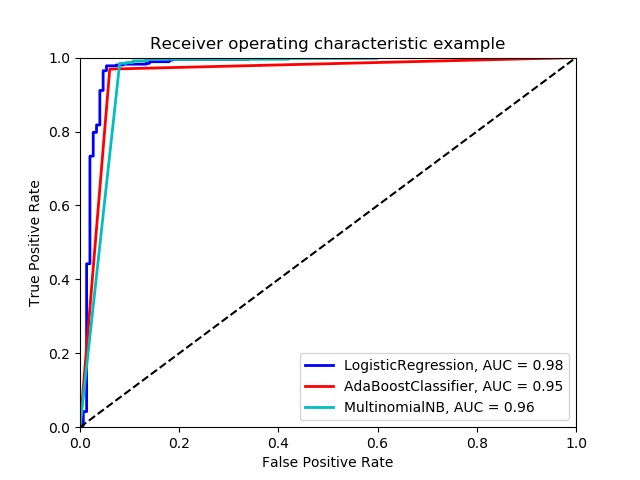
\includegraphics[width=2in]{roc.png}
%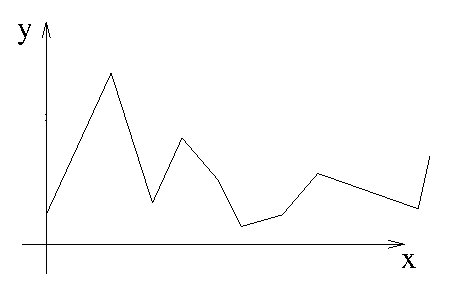
\includegraphics[width=2in]{figure.eps} %to texify use eps
\caption{Receiver Operating Characteristic curve (ROC curve)}
\end{center}
\label{fig:mypic}
\end{figure}
\end{enumerate}


%%%%%%%%%%%%%%%%%%%%%%%%%
%%%%%%%%%%%%%%%%%%%%%%%%%
\section{Conclusion}

In this paper, we propose four machine learning methods for spam filtering and present an empirical evaluation for them on data corpus given to us. These approaches include Logistic Regression classifier, AdaBoost classifier, Random Forest classifier and Naive Bayesian Classifier. The only one experiment, is carried out to test the performances of these algorithms by changing the values of the hyper-parameters with the use of an optimizer (grid search). Experimental results show that Random Forest classifier is more sensitive to the training set size and unsuitable for using as a spam filtering. Generally, the performances of the Logistic regression classifier and Naive Bayesian classifier are less influenced by data sets, and slightly superior to the AdaBoost classifier. Hence, we selected the logistic regression classifier as the final spam filtering. We also choose this one because it shows higher AUC which is also realted to the accuracy.


\begin{thebibliography}{1}
\bibitem{temp1}
https://gab41.lab41.org/the-10-algorithms-machine-learning-engineers-need-to-know-f4bb63f5b2fa
\bibitem{temp2}
https://towardsdatascience.com/the-random-forest-algorithm-d457d499ffcd
\end{thebibliography}

\end{document}



